In this section, we discuss the results achieved using our proposed offloading heuristics.
All experiments were conducted on a Galaxy Nexus S device and using an HP (Intel 64 bit) machine as a server.
We see a performance improvement
of up to 11\% on a synthetic application. Our results also include conducting the experiments with different bandwidth conditions.
\subsection{Parent-to-Native Heuristic Performance}
To evaluate the heuristics mentioned in Section~\ref{sec:smart_code} we implemented a synthetic application that performs mathematical computations and outputs the results at regular intervals. The idea behind choosing such an application is to emulate applications and benchmarks that perform compute intensive tasks and display intermediate results periodically in the progress bar (for instance, PI benchmark). We also analyzed our heuristics on Adobe's Photoshop Mobile application
(\texttt{com.adobe.psmobile}) since the image processing involved takes considerable amount of compute resources followed by displaying the resultant image to the user.

In order to automate the process of running photoshop, we wrote a UI testing script that generates action commands to change image aspects like exposure, soft focus, etc. several times. We observed that every exposure action command starts with native methods like nativeConfig, getNativePixels which run on the client, and is then followed by a compute intensive non-native method  (ExposureOp.LUTARGB) that allows the thread to be migrated in the base implementation. It was observed that on an average the thread was offloaded after two runs of exposure action in order to achieve the non-native execution time to be higher or equal to the threshold time based on sync time and the RTT. Our static profiling showed that ExposureOp.LUTARGB doesn't contain any native implementation and DDMS dynamic profiling listed this method as one of the methods with the largest execution time. Since every exposure ends with aborting the thread on the server and migrating back to the client, the performance improvement achieved by offloading fails to supersede the communication overhead encountered. Having access to the execution time from DDMS and the sync time from the network conditions and the state size, we were able to conclude that it is expensive to offload. Applying the Parent-to-Native heuristic, we prevent this method to offload and let the entire exposure thread run locally. As shown in Table~\ref{table:heuristic}, we observed an execution time improvement of 4.8\% in an experiment with 10 exposure commands that take a total of 83 secs in the baseline COMET implementation.  We also experimented by forcibly offloading this method on every run which led to significant performance degradation as shown in the table.

\subsection{Native-to-NextNative Heuristic Performance}
We next analyzed the performance improvement achieved by using the second heuristic mentioned in Section~\ref{sec:smart_code} on the synthetic application. The synthetic application has inter-leavings of native calls between the compute intensive tasks, which makes the server abort the thread when a native method is encountered. This native method is executed on the client and then gets offloaded back the to the server after a calculated period of time. The base implementation of COMET currently waits for non-native execution time to be twice the RTT which makes the resource hungry non-native method execute on the client for brief amount of time before it is offloaded. Our heuristic two annotates this method to be immediately offloaded giving us an overall performance improvement of over 11\% in the test run that took around x seconds as shown in Table~\ref{table:heuristic}

\subsection{Network Bandwidth Analysis}
In Section~\ref{sec:method} we explained the methodology used to retieve the current network bandwidth from the client. Once the client has information
about the size of data that needs to be sent over to the server, we compare it with the current bandwidth. We conducted our experiments with
different threshold values and evaluated the performance of applications. However, even after multiple experiments we were unable to see any
performance improvement over the current implementation. We believe the reason for this is the mechanism used to cancel the offloading decision at this point.
The size of data is to be transferred is computed after a lot of state is set up for thread migration. At this point, to revoke the
offloading decision the mechanism we used involved closing the socket to terminate connection to the server. Once this is done, the thread recovery mechanism
present in COMET performs a clean up and restores the state to the last safe point. The code then continues to execute locally on the client. The process
of invoking the thread recovery mechanism is not the best way to implement this as it might lead to additional overhead. However, due to
unfamiliarity with the internals of the COMET code base, we were unable to come up with a more efficient solution.


%-------------------------------------------------------%
\begin{figure} [thf*]
\centering
\begin{tabular}{c}
\begin{minipage}[b]{0.5\textwidth}
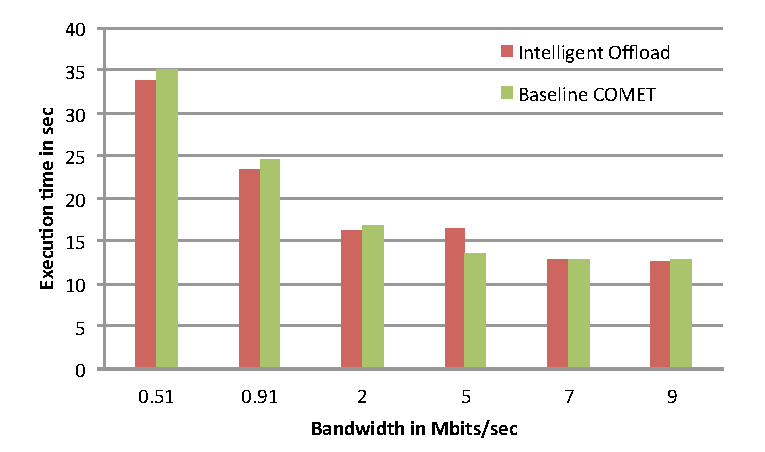
\includegraphics[width=0.95\textwidth]{figs/h1_sweep.pdf}
\end{minipage}
\end{tabular}
\caption{Execution results using the Parent-to-Native Heuristic for our synthetic application}
\label{fig:h1_sweep}
\end{figure}

%-------------------------------------------------------%
\begin{figure} [thf*]
\centering
\begin{tabular}{c}
\begin{minipage}[b]{0.5\textwidth}
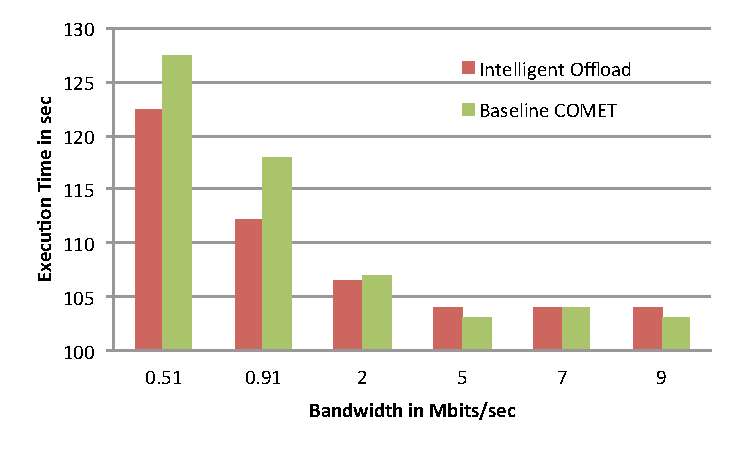
\includegraphics[width=0.95\textwidth]{figs/h2_sweep.pdf}
\end{minipage}
\end{tabular}
\caption{Execution results using the Native-to-NextNative Heuristic for our synthetic application}
\label{fig:h2_sweep}
\end{figure}

%-------------------------------------------------------------------------
\begin{table}[tbh]
{\small
\centering
\begin{minipage}{0.45\textwidth}
\centering
\begin{tabular}{|c|c|c|c|}
\hline
& Scientific Application & Photoshop \\
\hline
\hline
Parent-to-Native & 4.08 & 4.58\% \\ \hline
\hline
Native-to-NextNative & 11\%  & -24\%  \\ \hline
 \end{tabular}
\end{minipage}
\caption{Relative improvement of different heuristics over Baseline COMET}
\label{table:heuristic}
\vspace{-6mm}
}
\end{table}
%-------------------------------------------------------------------------




\ignore{
%-------------------------------------------------------%
\begin{figure*} [tbf*]
\centering
\begin{tabular}{cc}
\begin{minipage}[b]{0.5\textwidth}
\includegraphics[height=0.2\textheight]{figs/fbfly-thpt.pdf}
\center
\vspace{-4mm}
(a)
\end{minipage}
&
\begin{minipage}[b]{0.5\textwidth}
\includegraphics[height=0.2\textheight]{figs/fbfly-lat.pdf}
\center
\vspace{-4mm}
(b)
\end{minipage}
\end{tabular}
\caption{Network throughput and packet latency for a Flattened Butterfly topology.}
\label{fig:fbfly}
%\vspace{-2mm}
\end{figure*}
%-------------------------------------------------------%
}
